\chapter{Wykresy}
\label{ch:dodatekC-wykresy}
\section{Porównanie scenariuszy doboru parametrów algorytmu memetycznego}
\subsection{Funkcja Paviani}
\begin{figure}[h]
%\centering
  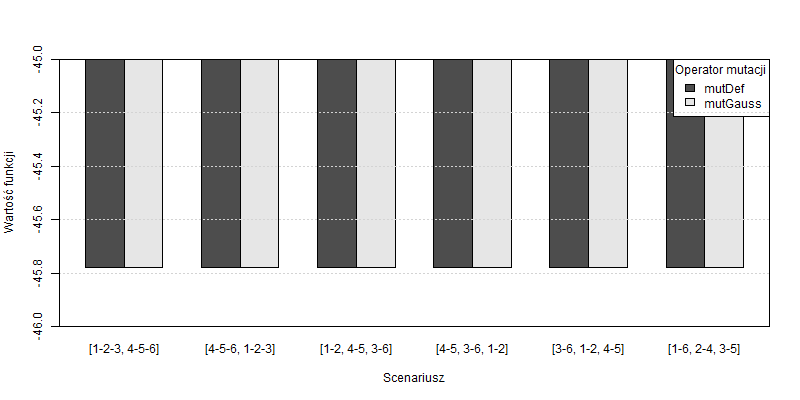
\includegraphics[width=\linewidth]{{img//app03//parameterSelection//bestfitness_calych_scenariuszy_Paviani.png}}
\caption{Porównanie najlepszego rozwiązania dla różnych scenariuszy dla funkcji Paviani}
\label{fig:app_parameter_selection_fitness_overall_paviani}
\end{figure}


\begin{figure}[h]
\centering
\begin{subfigure}{\textwidth}
  \centering
  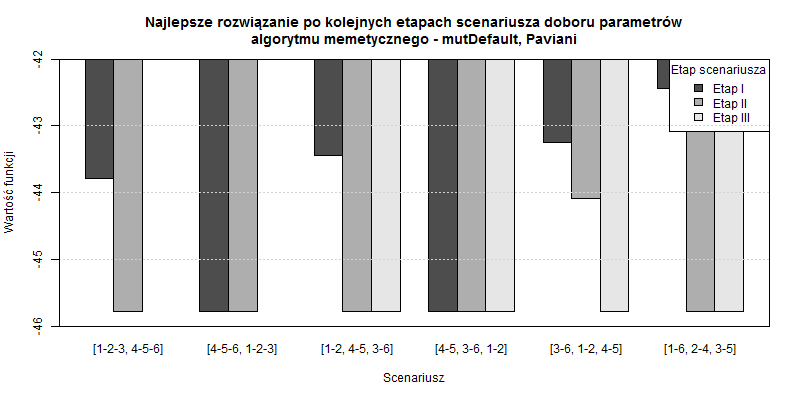
\includegraphics[width=\linewidth]{{img//app03//parameterSelection//fitness_etapow_scenariuszymutDefault_Paviani.png}}
  \caption{\emph{mutDefault}}
\end{subfigure}
\begin{subfigure}{\textwidth}
  \centering
  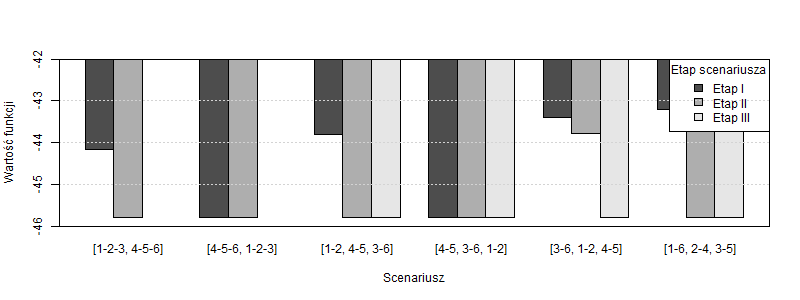
\includegraphics[width=\linewidth]{img//app03//parameterSelection//fitness_etapow_scenariuszymutGauss_Paviani.png}
  \caption{\emph{mutGauss}}
\end{subfigure}
\caption{Najlepsze znajdywane rozwiązanie kolejno w etapach selekcji dla funkcji Paviani}
\label{fig:app_parameter_selection_fitness_in_phases_paviani}
\end{figure}

%%%%%%%%%%%%%%%

\begin{figure}[h] 
\centering
  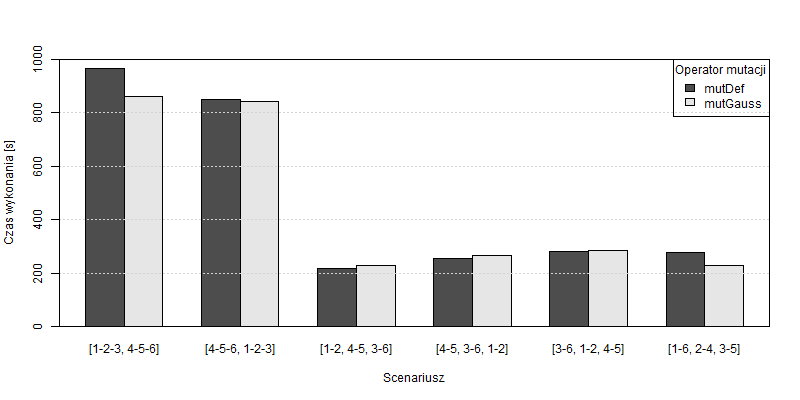
\includegraphics[width=\linewidth]{{img//app03//parameterSelection//czas_calych_scenariuszy_Paviani1.png}}
\caption{Czas wykonania różnych scenariuszy dla funkcji Paviani}
\label{fig:app_parameter_selection_time_overall_paviani}
\end{figure}


\begin{figure}[h] 
\centering
\begin{subfigure}{\textwidth}
  \centering
  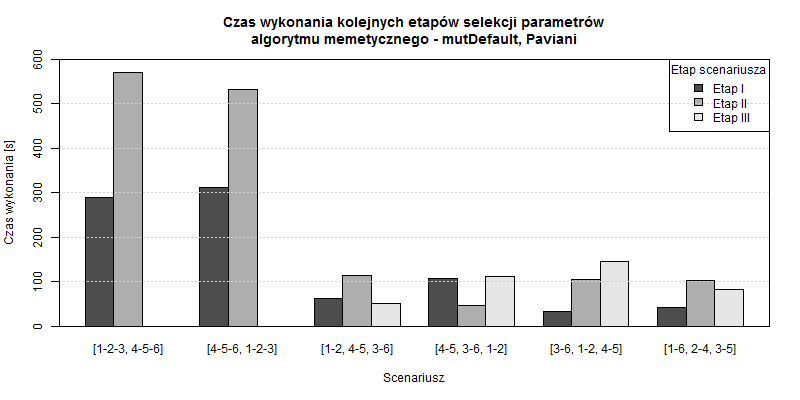
\includegraphics[width=\linewidth]{{img//app03//parameterSelection//czas_etapow_scenariuszymutDefault_Paviani.png}}
  \caption{\emph{mutDefault}}
\end{subfigure}
\begin{subfigure}{\textwidth}
  \centering
  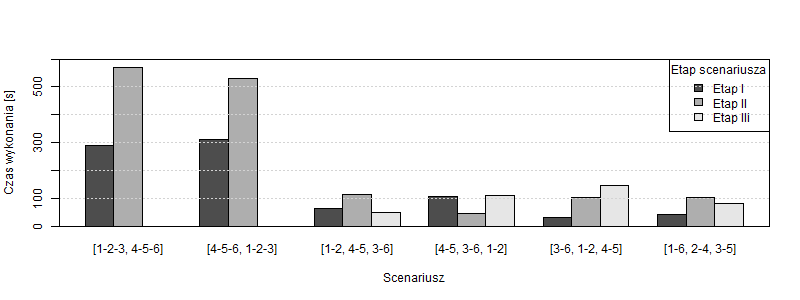
\includegraphics[width=\linewidth]{img//app03//parameterSelection//czas_etapow_scenariuszymutGauss_Paviani.png}
  \caption{\emph{mutGauss}}
\end{subfigure}
\caption{Czas wykonania kolejnych etapów selekcji dla funkcji Paviani}
\label{fig:app_parameter_selection_time_in_phases_paviani}
\end{figure}

\clearpage
%%%%%%%%%%%%%%%%%%%%%%%%%%%%%%%%%%%%%%%%%%%%%%%%%%%%%%%%%%%%%%%%%%%%%%%%%%%%%%%%%%%%%%%%%%%

\subsection{Funkcja ZeldaSine10}
\begin{figure}[h] 
\centering
  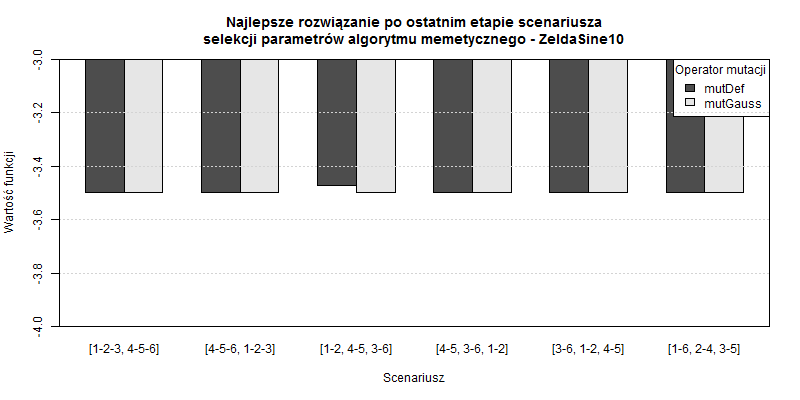
\includegraphics[width=\linewidth]{{img//app03//parameterSelection//bestfitness_calych_scenariuszy_ZeldaSine.png}}
\caption{Porównanie najlepszego rozwiązania dla różnych scenariuszy dla funkcji ZeldaSine10}
\label{fig:app_parameter_selection_fitness_overall_zeldasine}
\end{figure}


\begin{figure}[h]
\centering
\begin{subfigure}{\textwidth}
  %\centering
  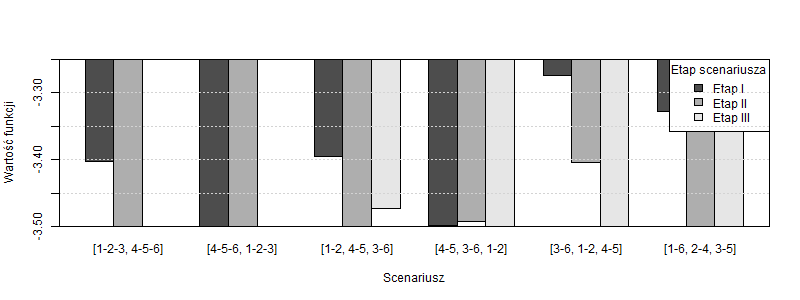
\includegraphics[width=\linewidth]{{img//app03//parameterSelection//fitness_etapow_scenariuszymutDefault_ZeldaSine10.png}}
  \caption{\emph{mutDefault}}
\end{subfigure}
\begin{subfigure}{\textwidth}
  %\centering
  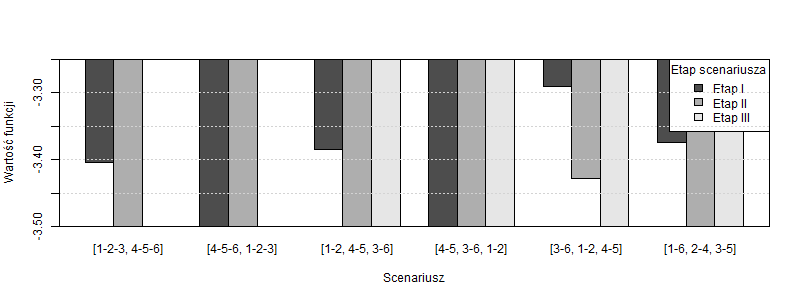
\includegraphics[width=\linewidth]{img//app03//parameterSelection//fitness_etapow_scenariuszymutGauss_ZeldaSine10.png}
  \caption{\emph{mutGauss}}
\end{subfigure}
\caption{Najlepsze znajdywane rozwiązanie kolejno w etapach selekcji dla funkcji ZeldaSine10}
\label{fig:app_parameter_selection_fitness_in_phases_zeldasine}
\end{figure}

%%%%%%%%%


\begin{figure}[h]
\centering
  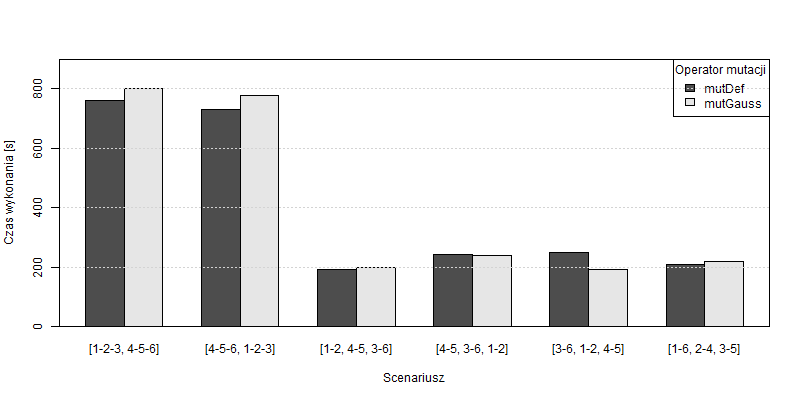
\includegraphics[width=\linewidth]{{img//app03//parameterSelection//czas_calych_scenariuszy_ZeldaSine10.png}}
\caption{Czas wykonania różnych scenariuszy dla funkcji ZeldaSine10}
\label{fig:app_parameter_selection_time_overall_zeldasine}
\end{figure}


\begin{figure}[h] 
\centering
\begin{subfigure}{\textwidth}
  %\centering
  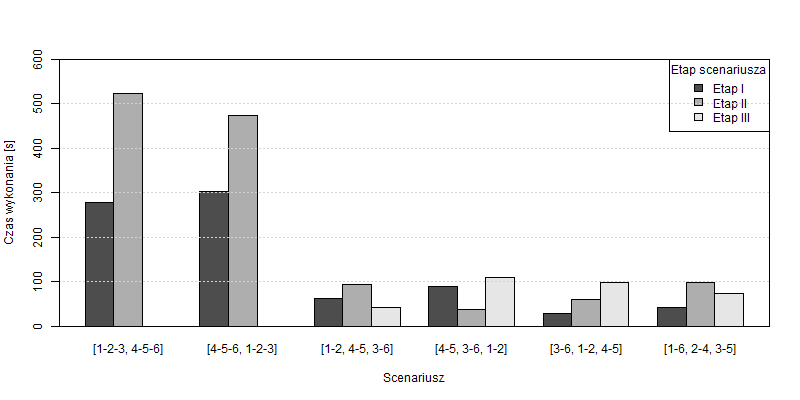
\includegraphics[width=\linewidth]{{img//app03//parameterSelection//czas_etapow_scenariuszymutDefault_ZeldaSine10.png}}
  \caption{\emph{mutDefault}}
\end{subfigure}
\begin{subfigure}{\textwidth}
  %\centering
  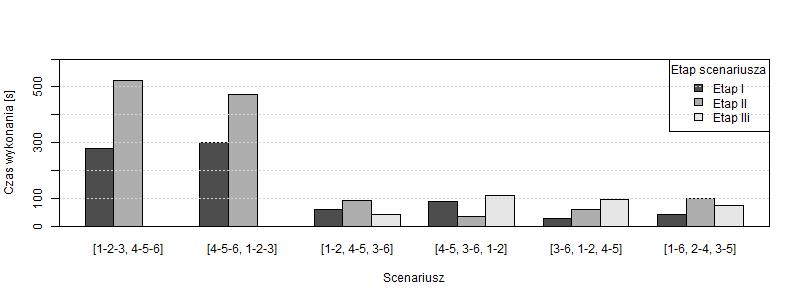
\includegraphics[width=\linewidth]{img//app03//parameterSelection//czas_etapow_scenariuszymutGauss_ZeldaSine10.png}
  \caption{\emph{mutGauss}}
\end{subfigure}
\caption{Czas wykonania kolejnych etapów selekcji dla funkcji ZeldaSine10}
\label{fig:app_parameter_selection_time_in_phases_zeldasine}
\end{figure}